% imports
\documentclass[titlepage]{article}
\usepackage[utf8]{inputenc}
\usepackage[a4paper, total={16cm, 23cm}, top=3.5cm]{geometry}
\usepackage[dvipsnames]{xcolor}
\usepackage{
    amsmath,
    amssymb,
    amsthm,
    fancyhdr,
    siunitx,
    bm,
    lipsum,
    standalone,
    tikz,
    booktabs,
    enumitem,
    array,
}
\usepackage[colorlinks=true, allcolors=linkcolor]{hyperref}
\usepackage[nameinlink]{cleveref}
\usepackage[
    backend=biber,
    bibstyle=ext-authoryear,
    citestyle=ext-authoryear-comp,
    sorting=nyt,
    uniquename=false,
    maxbibnames=99,
    giveninits=true,
]{biblatex}

% bibliographic options
\DeclareFieldFormat[article]{volume}{\mkbibbold{#1}}
\DeclareFieldFormat[article]{number}{\mkbibparens{#1}}
\DeclareFieldFormat[article]{pages}{#1}
\renewcommand*{\volnumdelim}{}
\renewbibmacro{in:}{}
\addbibresource{references.bib}
\DeclareFieldFormat{titlecase:title}{\MakeSentenceCase*{#1}}

% ref options
\crefname{section}{\S}{\S\S}
\crefname{subsection}{\S}{\S\S}
\crefname{equation}{}{}
\crefname{figure}{Figure}{Figures}
\newcommand\crefrangeconjunction{--}
\def\equationautorefname~#1\null{(#1)\null}
\numberwithin{equation}{section}
\definecolor{linkcolor}{RGB}{51, 54, 142}

\makeatletter
\patchcmd{\math@cr@@@align}{\cr}{\global\let\df@label\@empty\cr}{}{}
\makeatother

% page style options
\pagestyle{fancy}
\fancyhead{}
\rhead{Title}
\renewcommand{\headrulewidth}{0.5pt}
\setlength{\headheight}{15pt}
\setlength\parindent{0pt}
\setlength\parskip{6pt}

% math macros
\renewcommand{\d}[1]{\mathrm{d}#1}
\newcommand{\diff}[2]{\frac{\mathrm{d} #1}{\mathrm{d} #2}}
\newcommand{\ddiff}[2]{\frac{\mathrm{d}^2 #1}{\mathrm{d} {#2}^2}}
\newcommand{\pdiff}[2]{\frac{\partial #1}{\partial #2}}
\renewcommand\vec{\bm}
\newcommand{\uvec}[1]{\vec{\hat{#1}}}
\newcommand{\grad}{\vec{\nabla}}
\newcommand{\prandtl}{\ensuremath{\mathrm{Pr}}}
\newcommand{\rayleigh}{\ensuremath{\mathrm{Ra}}}
\newcommand{\nusselt}{\ensuremath{\mathrm{Nu}}}

% text macros
\newcommand{\rb}{Rayleigh-B\'{e}nard}

\begin{document}
\begin{titlepage}
\vfill~

\begin{center}
    {\Huge \textbf{%
        Title
    }} \\
    \vspace{0.75cm}
    {\Large\textbf{Honours Literature Review}} \\
    \vspace{0.75cm}
    {\Large\textbf{Thomas D. Schanzer}} \\
    \vspace{6pt}
    {\large Supervisor: Prof. Steven Sherwood} \\
    \vspace{0.75cm}
    {\large%
        School of Physics

        Climate Change Research Centre and
        ARC Centre of Excellence for Climate Extremes

        University of New South Wales, Sydney, Australia
    }
\end{center}
\vfill
\begin{center}
{\large\textbf{Abstract}}

\begin{minipage}{13cm}
    Text
\end{minipage}
\end{center}
\vfill
\end{titlepage}

\newpage
\tableofcontents

\newpage
\pagestyle{fancy}
\thispagestyle{fancy}

\section{Introduction}
\subsection{Traditional parametrisation schemes}

\section{Theory of parametrisation}

\section{Data-driven parametrisation schemes}

\section{Parametrisation development using toy models}

\newpage
\section{\rb{} convection and numerical considerations}
\subsection{Problem statement}
\rb{} convection is the motion of a fluid confined between two
horizontal isothermal plates, the temperature of the bottom plate being
higher than that of the top plate. The governing equations for the flow
follow from the Navier-Stokes equations of mass, energy and momentum
conservation. The reader is referred to \textcite{chandrasekhar1961} for
a detailed derivation; I summarise the assumptions and approximations
involved below.

The density, $\rho$, of the fluid is related to its temperature $T$ by
the linear equation of state
\[
    \rho = \rho_0 [1 - \alpha(T - T_0)],
\]
where $\alpha$ is the (constant) volume coefficient of thermal expansion and
$\rho_0$ and $T_0$ are the base-state density and temperature such that $\rho =
\rho_0$ when $T = T_0$. The key assumption is that density variations are small
($\alpha (T - T_0) \ll 1$), which allows the governing equations to be
simplified under the \emph{Boussinesq approximation}. The Boussinesq
approximation involves first writing the pressure, $p$, of the fluid as
\[
    p = p_0 - \rho_0 gz + p',
\]
where $p_0$ is an arbitrary constant, $g$ is the acceleration due to gravity
and $z$ is the vertical coordinate. $p'$ is the (time-varying) deviation from
a hydrostatically balanced background profile $p_0 - \rho_0 gz$
in which the upward pressure gradient force per unit volume $\rho_0 g$ cancels
the downward weight force per unit volume $-\rho_0 g$. Since
$\alpha (T - T_0) \ll 1$, density variations are neglected everywhere except
in their contribution to the weight force, leading to a net buoyant
(background pressure gradient plus weight) force per unit mass
\[
    \frac{\rho_0 - \rho}{\rho_0} g = \alpha (T - T_0) g.
\]

With these assumptions in mind, I adopt the governing equations as they
are derived by \textcite{chandrasekhar1961}:
\begin{alignat}{2}
    \label{eqn:dim_momentum}
    \pdiff{\vec{u}}{t} + \vec{u} \cdot \grad \vec{u}
        &= -\frac{1}{\rho_0} \grad p' + \alpha (T - T_0) g \uvec{z}
        + \nu \nabla^2 \vec{u}
    &\quad& \text{(momentum conservation),} \\
    \label{eqn:dim_energy}
    \pdiff{T}{t} + \vec{u} \cdot \grad T
        &= \kappa \nabla^2 T
    && \text{(energy conservation), and} \\
    \label{eqn:dim_incompressible}
    \grad \cdot \vec{u} &= 0
    && \text{(incompressibility).}
\end{alignat}
$\vec{u}$ is the fluid velocity, $t$ is time, $\uvec{z}$ is the upward
unit vector, $\nu$ is the (constant) kinematic viscosity and $\kappa$ is
the thermal diffusivity (also constant). Notice that the aforementioned
buoyancy term $\alpha (T - T_0) g$ appears on the right-hand side of
\cref{eqn:dim_momentum}.

The parametrisation test-bed developed in this work solves the governing
equations in a two-dimensional domain $(x,z) \in [0, d] \times [0, L]$, subject
to no-slip, isothermal boundary conditions on the top and bottom plates,
\begin{alignat}{3}
    \label{eqn:dim_bc_bot}
    \vec{u} &= \vec{0}, &\quad T &= T_0 + \frac{\delta T}{2}
    &\qquad& \text{at } z = 0 \text{ and} \\
    \label{eqn:dim_bc_top}
    \vec{u} &= \vec{0}, &\quad T &= T_0 - \frac{\delta T}{2}
    &\qquad& \text{at } z = d,
\end{alignat}
and periodic boundary conditions in the horizontal,
\begin{alignat}{2}
    \label{eqn:dim_bc_sides}
    \vec{u}(x=0) &= \vec{u}(x=L) &\quad \text{and} \quad T(x=0) &= T(x=L).
\end{alignat}
$\delta T$ is the constant temperature difference between the plates.

\subsection{Nondimensionalisation and scale analysis}
It is helpful to nondimensionalise the governing equations
\crefrange{eqn:dim_momentum}{eqn:dim_bc_sides}; this is not only useful
for numerical work but also gives insight into the different flow
regimes that are possible. A range of nondimensionalisations are used in
fluid dynamics literature; I adopt a common one (see, e.g.,
\textcite{grotzbach1983,ouertatani2008,stevens2010}) which is suitable
for the turbulent convective regime.

For low-viscosity, turbulent flow, a suitable time scale is the
\emph{free-fall time} $t_0$, which is the time for a fluid element with
constant temperature $T = T_0 - \delta T$ to fall from the top plate to
the bottom plate under the influence of buoyancy ($-g \alpha \delta T$)
alone. It is simple to show that
\[
    t_0 \sim \left( \frac{d}{g \alpha \delta T} \right)^{1/2},
\]
ignoring a factor of $\sqrt{2}$. The obvious length and temperature
scales are the plate separation $d$ and temperature difference $\delta T$,
respectively.

Making the substitutions $p'/\rho_0 \to \pi$ and $T - T_0 \to \theta$
in \crefrange{eqn:dim_momentum}{eqn:dim_bc_sides} and expressing all
variables in units of $t_0$, $d$ and $\delta T$ leads to the dimensionless
equations
\begin{align}
    \label{eqn:momentum}
    \pdiff{\vec{u}}{t} + \vec{u} \cdot \grad \vec{u}
        &= -\grad \pi + \left( \frac{\prandtl}{\rayleigh}\right)^{1/2}
        \nabla^2 \vec{u} + \theta \uvec{z}, \\
    \label{eqn:energy}
    \pdiff{\theta}{t} + \vec{u} \cdot \grad \theta
        &= (\rayleigh\,\prandtl)^{-1/2} \, \nabla^2 \theta, \quad \text{and} \\
    \label{eqn:incompressible}
    \grad \cdot \vec{u} &= 0,
\end{align}
with boundary conditions
\begin{gather}
\begin{alignat}{3}
    \label{eqn:bc_bot}
    \vec{u} &= \vec{0}, &\quad \theta &= +\frac{1}{2}
    &\qquad& \text{at } z = 0, \\
    \label{eqn:bc_top}
    \vec{u} &= \vec{0}, &\quad \theta &= -\frac{1}{2}
    &\qquad& \text{at } z = 1,
\end{alignat} \\
\begin{alignat}{2}
    \label{eqn:bc_sides}
    \vec{u}(x=0) &= \vec{u}(x=\Gamma)
    &\quad \text{and} \quad \theta(x=0) &= \theta(x=\Gamma).
\end{alignat}
\end{gather}
There are three dimensionless parameters: the aspect ratio of the domain
\[
    \Gamma \equiv \frac{L}{d},
\]
the \emph{Prandtl number}
\[
    \prandtl \equiv \frac{\nu}{\kappa}
\]
which measures the relative importance of viscosity (momentum diffusivity)
and thermal diffusivity, and the \emph{Rayleigh number}
\[
    \rayleigh \equiv \frac{g \alpha d^3 \delta T}{\kappa \nu}.
\]
The Rayleigh number can be interpreted as the ratio of the time scale for
thermal transport by convection to the time scale for thermal transport by
conduction. It determines the importance of diffusion for the evolution of
$\vec{u}$ and $\theta$; inspection of \cref{eqn:momentum,eqn:energy} indicates
that low $\rayleigh$ implies strong diffusion and high $\rayleigh$ weak
diffusion. Detailed theoretical analysis of the governing equations (see, e.g.,
\textcite{chandrasekhar1961} and the seminal work by \textcite{rayleigh1916})
reveals that there exists a critical Rayleigh number (dependent on boundary
conditions but of order $\SI{e3}{}$), below which the equations have a stable
equilibrium with the fluid at rest and a linear conductive temperature profile.
Above the critical value, the equilibrium is unstable and small perturbations
lead to the formation of a regular series of steady, rotating convection cells.
If the Rayleigh number is increased much further (\textcite{le_quere1991} cites
$\rayleigh \approx \SI{2e8}{}$), the solution becomes unsteady and increasingly
turbulent. This work is concerned with the turbulent regime, since Rayleigh
numbers for atmospheric deep moist convection can be as large as $\SI{e22}{}$
\parencite{chilla2012}.

\subsection{Resolution dependence of numerical solutions}
In constructing a parametrisation test-bed, I will firstly seek
reasonably accurate, high-resolution ``truth'' solutions of
\crefrange{eqn:momentum}{eqn:bc_sides}. I will then deliberately reduce
the resolution, aiming to produce solutions that are sufficiently
``different'' that they might reasonably be ``improved'' by a parametrisation
scheme. In this section, I review relevant literature with the aim of
establishing how, exactly, under-resolved simulations of \rb{} convection
might ``differ'' from well-resolved ones, and thus what one would hope to
``improve''. Specifically, I will address the following questions:
\begin{itemize}
    \item What resolution is necessary for a converged solution?
    \item Which quantities are most sensitive to insufficient resolution?
\end{itemize}

\subsubsection{Aside: Nusselt number and thermal boundary layer thickness}
The rate of heat transport across the fluid layer has physical significance for
natural realisations of thermally driven convection. It is widely analysed in
terms of the dimensionless \emph{Nusselt number}, whose accurate determination
is a common theme in the \rb{} convection literature; I therefore introduce
this quantity before proceeding. The Nusselt number measures the rate of
(vertical) heat transport across a horizontal plane at height $z$, normalised
by the purely conductive rate that would exist if the fluid were at rest
\parencite{verzicco1999}. Following \textcite{chilla2012}, I use the definition
(before nondimensionalisation)
\begin{equation}
    \label{eqn:dim_nusselt}
    \nusselt(z,t) \equiv \frac{
        \langle wT \rangle_A - \kappa \partial \langle T \rangle_A / \partial z
    }{
        \kappa \delta T / d
    }
\end{equation}
where $\langle \cdot \rangle_A$ denotes averaging over the horizontal
plane at height $z$ and $w = \vec{u} \cdot \uvec{z}$ is the vertical
velocity. The rate of heat transport in the numerator has two terms:
advection $\langle wT \rangle_A$ and conduction
$-\kappa \partial \langle T \rangle_A / \partial z$. The denominator
$\kappa \delta T / d$ is the rate of heat transport for a linear
conductive temperature profile with the fluid at rest.
\textcite{scheel2013} give the corresponding nondimensionalised form,
\begin{equation}
    \label{eqn:nusselt}
    \nusselt(z,t) \equiv (\rayleigh\,\prandtl)^{1/2} \langle w \theta \rangle_A
        - \pdiff{\langle \theta \rangle_A}{z}.
\end{equation}

Another important quantity is the thickness of the \emph{thermal boundary
layer} at each plate where large temperature gradients exist.
\textcite{chilla2012} outline the method for estimating $\delta_T$: if, on
average, the fluid temperature changes with height from $+\delta T/2$ at the
lower plate to $0$ (the mean value in the well-mixed interior) over a distance
$\delta_T$, then
\[
    \left. \pdiff{\langle T \rangle_A}{z} \right|_{z=0}
        \approx -\frac{\delta T}{2 \delta_T}.
\]
But if one considers the definition of the Nusselt number
\cref{eqn:dim_nusselt} at $z=0$, the advection term $\langle wT \rangle_A$
vanishes due to the $\vec{u} = \vec{0}$ boundary condition and
\[
    \nusselt(z=0) = -\frac{d}{\delta T}
        \left. \pdiff{\langle T \rangle_A}{z} \right|_{z=0}.
\]
Thus,
\begin{equation}
    \label{eqn:thermal_bl}
    \delta_T = \frac{d}{2\,\nusselt(z=0)}.
\end{equation}

\subsubsection{Theoretical resolution requirements for accurate simulations}%
\label{sec:res_requirements}

% resolution in general, Grotzbach condition.
\textcite{grotzbach1983} is recognised as the first to formulate resolution
requirements for accurate simulations of \rb{} convection
\parencite{chilla2012,scheel2013}. He identified separate constraints on the
mean (i.e., averaged in each spatial direction) grid spacing and the vertical
spacing near the plates; we first discuss the former.
\citeauthor{grotzbach1983} reasoned that a numerical model that neglects
subgrid-scale effects must have a geometric mean grid spacing $h = (\Delta x
\Delta y \Delta z)^{1/3}$ such that
\begin{equation}
    \label{eqn:grotzbach}
    h \leq \pi \eta = \pi \left(
        \frac{\nu^3}{\langle \epsilon \rangle}
    \right)^{1/4}
\end{equation}
where $\eta \equiv (\nu^3/\epsilon)^{1/4}$ is the \emph{Kolmogorov length}, the
universal smallest relevant length scale for general turbulent flow, and
$\langle \epsilon \rangle$ is the spatial and temporal average of the kinetic
energy dissipation rate defined by
\begin{equation}
    \label{eqn:kinetic_dissipation}
    \epsilon(\vec{x}, t) \equiv \frac{\nu}{2} \sum_{ij} \left(
        \pdiff{u_i}{x_j} + \pdiff{u_j}{x_i}
    \right)^2
\end{equation}
\parencite{chilla2012}. The condition \cref{eqn:grotzbach} can be
understood using the Nyquist-Shannon theorem, which states that a
sampling frequency $f \geq k/\pi$ is needed to unambiguously reconstruct
a signal with wavenumber $k$; substituting $f = 1/h$, $k = 1/\eta$ leads
to the claimed relation.

% resolution near plates, number of points.
\citeauthor{grotzbach1983} recognised that the above reasoning was only valid
for the mean grid spacing; large gradients in temperature and velocity near the
top and bottom plates require finer resolution in those regions. The notion of
nearness can be formalised using the thermal boundary layer thickness
\cref{eqn:thermal_bl}, and one asks how many grid points are necessary in this
layer. \citeauthor{grotzbach1983} did not give a theoretical argument to derive
this number but claimed that 3 points are sufficient for turbulent flows.
\textcite{shishkina2010} presented a theoretical argument based on the
(experimentally and numerically justified) assumption of laminar
\emph{Prandtl-Blasius} flow conditions in the boundary layer and were able to
calculate the minimum number of grid points (e.g., 9 for $\rayleigh =
\SI{2e9}{}$ and $\prandtl = 0.7$). The results agreed with criteria derived in
previous numerical experiments. Importantly, the results of
\citeauthor{shishkina2010} allow \emph{a priori} determination of vertical
resolution requirements, potentially bypassing the time-consuming and expensive
process of iteratively running simulations, checking their convergence and
updating the resolution.

\subsubsection{
    Resolution-dependence tests and consequences of under-resolution}%
\label{sec:res_tests}

Performing numerical experiments for a 3D fluid layer,
\citeauthor{grotzbach1983} found that RMS velocity and Nusselt number were
the most sensitive quantities to insufficient mean grid spacing, but even
they increased ``only slightly'' above the values obtained from well-resolved
simulations. He concluded that condition \cref{eqn:grotzbach} was overly
restrictive and recommended (for $\prandtl > 0.59$) the simplified,
approximate version
\[ % is this necessary?
    h \lesssim 5.23 \, \prandtl^{-1/4} \rayleigh^{-0.3205}.
\]
Later work also supports the finding that the Nusselt number is
sensitive to under-resolution. Even studying only steady-state convective
solutions at moderate Rayleigh number, \textcite{le_quere1991} found that the
maximum and minimum Nusselt numbers were most sensitive to changes in
resolution and had the largest uncertainty among existing benchmark solutions.
% ouertatani: common to use Nu as convergence test
Other studies have used the convergence of the Nusselt number as an indicator
that the spatial resolution is sufficient to produce an accurate solution
\parencite{ouertatani2008}.

\textcite{stevens2010} performed 3D simulations in a finite cylindrical cavity
with the aim of reconciling the apparent disagreement between the Nusselt
numbers in previous numerical studies and experimental observations. They found
that agreement with experiment could be achieved, but only by using a much
higher resolution than the previous studies. They offered the physical
explanation that horizontally under-resolved simulations produce insufficient
thermal diffusion, leading to systematic overestimation of the buoyancy of
convective plumes near the side-walls of the cylinder; this results in Nusselt
numbers that exceed experimentally observed values. This led them to conclude
that the two criteria of \textcite{grotzbach1983}---for mean grid spacing
and for the vertical spacing near the upper and lower plates---are not
independent; the definition $h = (\Delta x \Delta y \Delta z)^{1/3}$ in
\cref{eqn:grotzbach} allows the horizontal spacing to remain relatively
coarse near the plates, provided the vertical spacing is small. Since
fine horizontal resolution is also necessary to accurately capture
the dynamics of the thin plumes, they proposed that \cref{eqn:grotzbach} be
applied with $h = \max(\Delta x, \Delta y, \Delta z)$ instead.

% kooij: Nu may not be best indicator
Some more recent work, however, casts doubt on the notion that the Nusselt
number is sensitive to under-resolution and that its convergence is a good
indicator that the flow is well-resolved. In assessing the performance of
several published computational fluid dynamics codes on the \rb{} problem in a
cylindrical cavity, \textcite{kooij2018} identified one higher-order code that
reproduced the theoretically predicted scaling of $\nusselt$ as a function of
$\rayleigh$ even when the flow was deliberately under-resolved. On the other
hand, the presence of numerical artefacts in the instantaneous temperature
field near the bottom plate was a clear indicator of insufficient resolution.
\cref{fig:kooij2018_artefacts}, a reproduction of part of their Figure 5, shows
these artefacts.

% scheel: dissipation rates sensitive
\textcite{scheel2013} performed similar high-resolution simulations for
a cylindrical cavity and also found that the Nusselt number, among other
global transport properties, were ``fairly insensitive to insufficient
resolution, as long as the mean Kolmogorov length [was] resolved'' (i.e.,
\cref{eqn:grotzbach} was satisfied). However, they found that the horizontally
averaged or local kinetic energy dissipation rate
\cref{eqn:kinetic_dissipation} and the corresponding thermal dissipation rate
\begin{equation}
    \label{eqn:thermal_dissipation}
    \epsilon_T(\vec{x}, t) \equiv \kappa \sum_i \left(\pdiff{T}{x_i}\right)^2
\end{equation}
were much more sensitive, with their convergence requiring even stricter
conditions than \cref{eqn:grotzbach}.

\begin{figure}[ht]
    \centering
    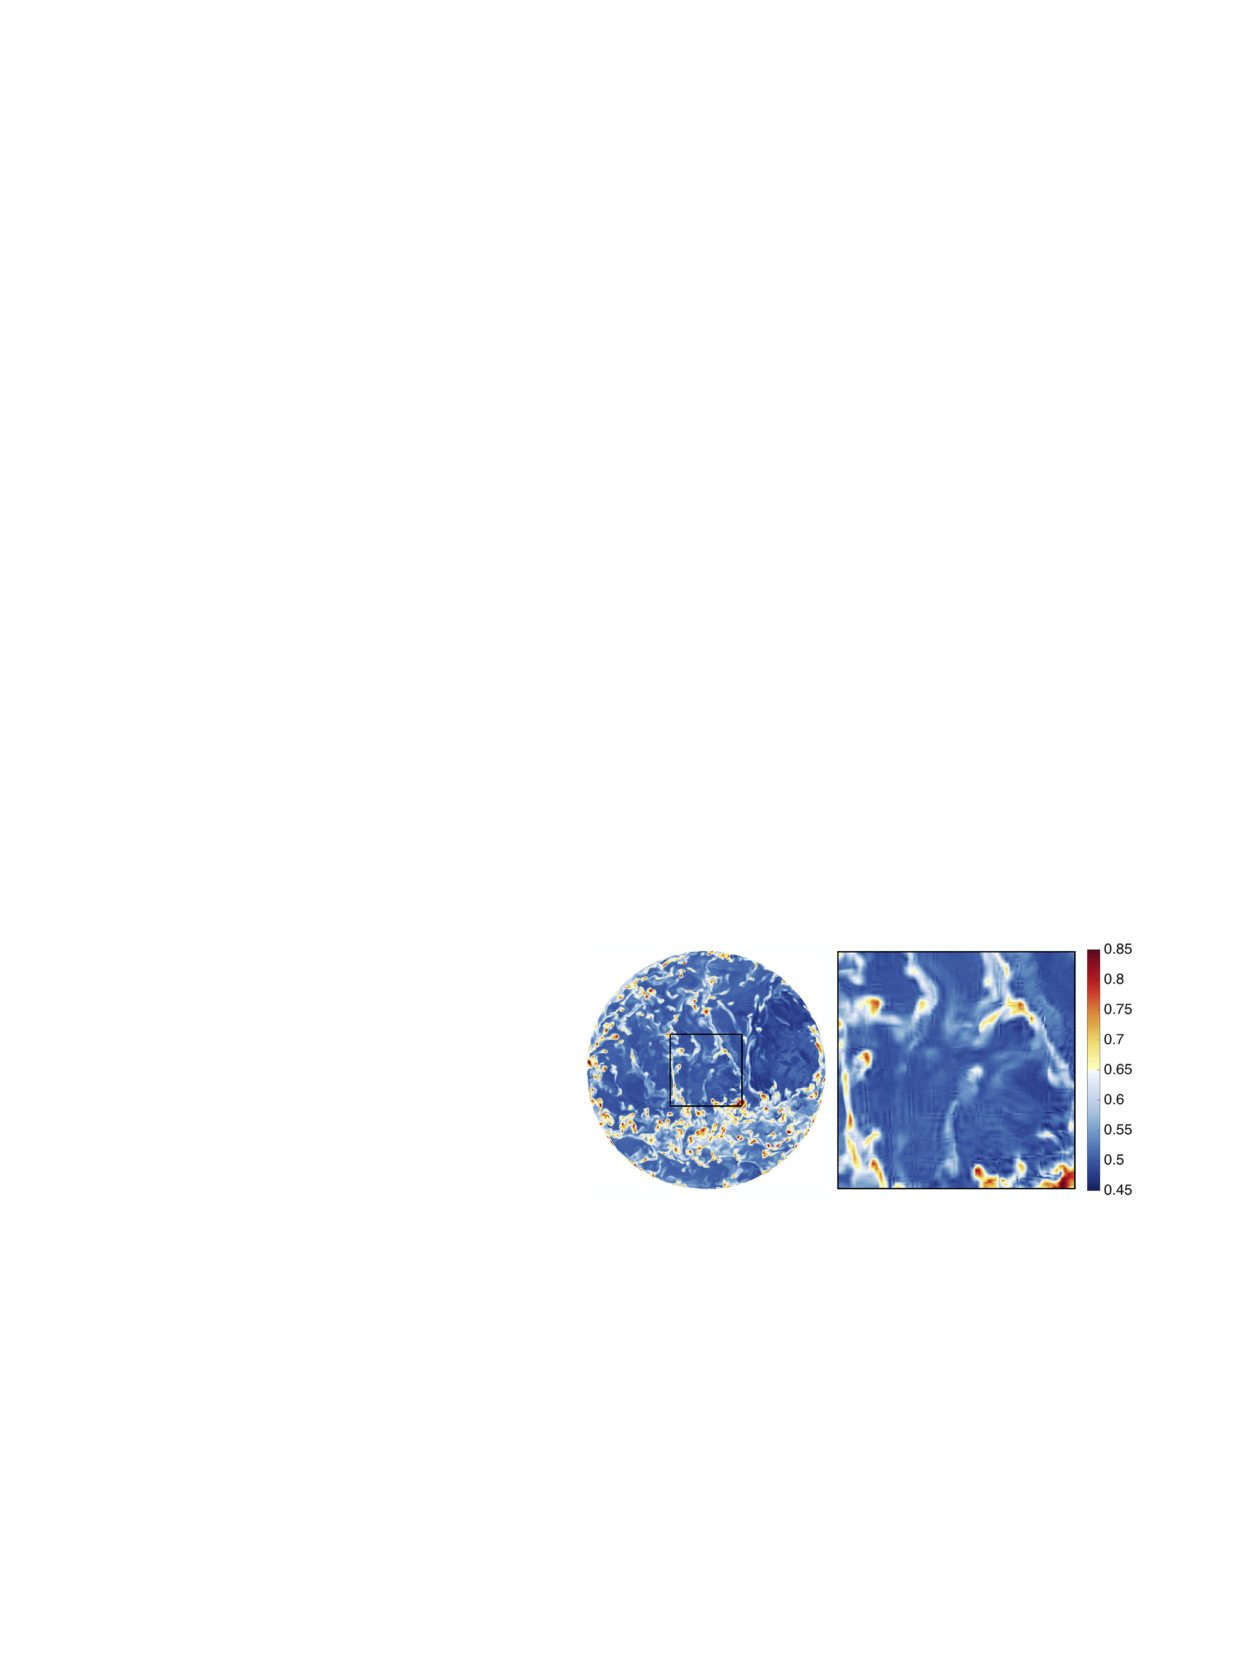
\includegraphics[width=\linewidth]{figures/kooij2018_artefacts.pdf}
    \caption{
        Reproduction of part of Figure 5 by \textcite{kooij2018}, showing an
        instantaneous horizontal temperature profile simulated by the
        \textsc{Nek}5000 code for \rb{} convection at $\rayleigh =
        \SI{e10}{}$. The profile is taken near the bottom plate of a
        cylindrical cavity and shows a grid-like pattern of numerical
        artefacts. The right panel is an enlargement of the region inside
        the black square in the left panel.
    }
    \label{fig:kooij2018_artefacts}
\end{figure}

\newpage
\section{Conclusion}

\newpage
\emergencystretch=5em
\printbibliography
\end{document}
